\documentclass{beamer}
\usetheme{Warsaw}
\useinnertheme{umbcboxes}

\title{Taking the 'defunct' out of 'defunctionalization'}
\subtitle{And putting the 'fun' back in 'defunct'}

\author{Benjamin Schulz}

%%%%

\usepackage{amsmath}
\usepackage{proof}

\newcommand{\forget}[1]{}

\newcommand{\throw}[0]{\textsf{throw}}
\newcommand{\catch}[0]{\textsf{catch}}
\newcommand{\sloop}[0]{\textsf{loop}}
\newcommand{\sbreak}[0]{\textsf{break}}
\newcommand{\ifz}[0]{\textsf{ifzero}}
\newcommand{\jsr}[0]{\textsf{jsr}}
\newcommand{\rtid}[0]{\textsf{r$_{tid}$}}
\newcommand{\rparent}[0]{\textsf{r$_{parent}$}}
\newcommand{\rpc}[0]{\textsf{r$_{pc}$}}
\newcommand{\switcha}[0]{\textsf{switch}_{A}}
\newcommand{\switchz}[0]{\textsf{switch}_{Z}}
\newcommand{\kcreate}[0]{ \textsf{tcreate}$_{kernel}$}
\newcommand{\ucreate}[0]{  \textsf{tcreate}$_{user}$}


%%%%

\begin{document}

\maketitle{}

%%%% slide
\begin{frame}{What's the Big Picture? What's the Problem?}


\structure{Architecture: Major Passes of the CT Compiler}{
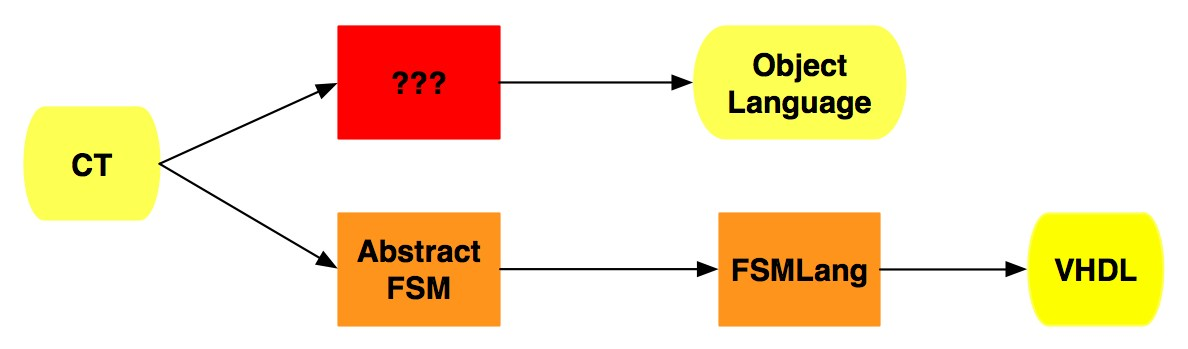
\includegraphics[width=4.0in]{compiler_diagram.jpg}}

\pause

\structure{... and architecture of what needs to be done}{
\begin{itemize}

\item{Rigorous definition of semantics for CT}
\item{Rigorous semantics of intermediate form}
\item{Construct well-defined relation between the two}
\item{Define compilation rules based on relation between CT and intermediate form}
\item{\emph{Overall, make design decisions that facilitate verification and correct code generation}}


\end{itemize}

} % end structure

\end{frame}


%%%% slide

\begin{frame}{Intermediate Language: Design Objectives}

\begin{itemize}

\item{Specification -- one we can stick with!}
  

\item{Implementation}

  \begin{itemize}
  
  \item{Write a code generation module that reflects the simulation relation between CT semantics and the OPSEM}
  
  \item{Construct a language to serve as a reasonable jumping-off point for generation of Microblaze-ready code, e.g. C or MB ASM}
    
  \end{itemize}


\item{Verification}

  \begin{itemize}
  
  \item{Preserve the resumption-monadic semantics of the CT source}
  
  \item{Establish a formal relation between a CT program and its intermediate form}
  
  \end{itemize}
  
\item{Application}
  \begin{itemize}
    \item{Produce working examples of secure, verifiable embedded system kernels}
  \end{itemize}
  
\end{itemize}


\end{frame}


%%%%% slide


\begin{frame}{Previous Attempts}

\begin{itemize}

\item{\Large{\color{blue}{In the beginning: TIC \cite{Palsberg_Ma_2002}}}}
  \begin{itemize}
  \item{i.e. the Typed Interrupt Calculus}
  \item{a language of interrupts and conditional atomicity}
  \end{itemize}
  
  \medskip

\item{\Large{\color{blue}{ETIC}}}
  \begin{itemize}
  \item{C with 'pthreads' primitive}
  \item{TIC+?}
  \end{itemize}

\medskip

\item{\Large{\color{blue}{OESS}}}
  \begin{itemize}
  \item{CT without monad operations}
  \item{... and with jumps, status registers}
  \item{ETIC+?}
  \end{itemize}

\medskip

\item{\Large{\color{blue}{The CHEAP Machine}}}
  \begin{itemize}
  \item{stab at an operational semantics}
  \item{closer to a typed assembly language}
  \item{ETIC++?}
  \end{itemize}
  
  \pause

\item{\emph{\color{red}{{Where's the 0xDEADBEEF?}}}}

\end{itemize}

\end{frame}

%%%%% slide
\begin{frame}{First Attempt: ETIC}

\structure{ETIC: Closest thing so far to code generation in action}{
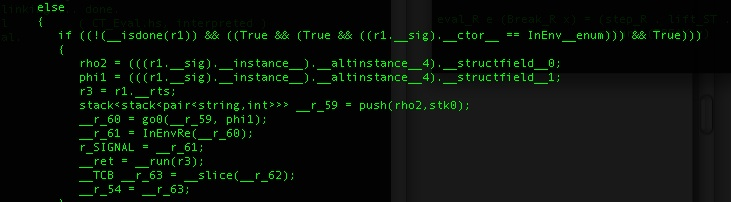
\includegraphics[width=3.9in]{etic_out_screen.jpg}
} % end structure

\structure{Virtues}{

  \begin{onlinebox}{9cm}
  
    \begin{itemize}
    
    \item{Working implementation of generation to MB}
    \item{Running kernel examples exist}
    \item{Easy to compile to C}
    
    \end{itemize}
  
  \end{onlinebox}

} % end structure

\smallskip

\structure{Vices}{

  \begin{onlinebox}{9cm}
  \begin{itemize}
 
  \item{Code generation ( :: CT $\rightarrow$ ETIC) is b0rk3d}
  
  \item{Informal semantics, difficulty squaring with CT}
  
  \item{Syntax obscures essential features}
  
  \end{itemize}
  \end{onlinebox}

} % end structure

\end{frame}


%%%%% slide
\begin{frame}{Second Attempt: OESS}

\structure{The Operational Execution Stream Semantics (OESS) Grammar}{

\begin{onlinebox}{11cm}

%begin syntax figure:

\begin{tabular*}{10cm}[]{cc}
{
\begin{minipage}[t]{1.85in}

\tiny{

$
\begin{array}[t]{lcl}


S &::=& A \ \textsf{;} \ S \ \mid \ \textsf {ifzero} \ S \ S \ S \ \mid \ \textsf {jsr} \ L \ S\\
  & \mid & \textsf {loop} \ S \ S \ \mid \ \textsf {done} \ X\\
  \\
A &::=& \textsf {atom(} K \textsf {)}\\
  &\mid & \textsf{tcreate}_{kernel} \ S\ \mid \ \textsf{tcreate}_{user} \ T\\
  &\mid & \textsf{kill} \ X \ \mid \ \textsf{catch} \ X \ L\\
  &\mid & \textsf{switch}_{A} \ X\ \mid \ \textsf{switch}_{Z} \ X\ \mid \ \textsf{break}\\
  \\
T &::=& \textsf{cont(} K\textsf{) \ ;} \ T \ \mid \ \textsf{throw(} X\textsf{) \ ;} \ T \\
  &\mid & \textsf {ifzero} \ T \ T \ T\ \ \mid \ \textsf {jsr} \ L \ T\\
  & \mid & \textsf {loop} \ T \ T\ \mid \ \textsf {done} \ X\\
  
\\
\end{array}
$

}  % end fontsize

\end{minipage}
}

{
\begin{minipage}[t]{1.85in}

\tiny{

$
\begin{array}[t]{lcl}

  M &::=& R \ \textsf{:=} \ X\ \mid \ \textsf{tst} \ X\ \mid \  \textsf{nop}\\
  K &::=& M\ \textsf{;}\ K \ \mid \ \ifz \ K \ K \ K \ \mid \ \jsr \ L \ K \mid M\\
\\
X &::=& R\ \mid \ L\\
  & \mid & \textsf{-}X\  \mid \ X \ \textsf{+} \ X \ \mid X \ \textsf{-} \ X\\
  & \mid & X \ \textsf{*} \ X \ \mid X \ \textsf{/} \ X\\
  & \mid & \textsf{!}X\  \mid \ X \ \textsf{\&\&} \ X \ \mid \ X \ \textsf{$\mid \mid$} \ X\\
  & \mid & Int\ \mid \ \textsf{nil}\\
  \\
R &::=& Var\  \mid \ Var \textsf{[}X\textsf{]}\\
  & \mid & \textsf{r$_{ret}$}\ \mid  \textsf{r$_{pc}$}
  \mid \  \textsf{r$_{signal}$}\  \mid  \textsf{r$_{tct}$} \mid  \textsf{r$_{Z}$}\\
  \\
  L &::=& Label\\
  
  \\
\end{array}
$

} % end fontsize

\end{minipage}
}


\\
\end{tabular*}

% end syntax figure

\end{onlinebox}

} %end structure


\structure{A typical transliteration CT $\rightarrow$ OESS}{

\begin{tabular}[t]{lll}

\begin{minipage}[t]{3.0cm}
$step_{R}\ k\ \bigstar_{R}\ \lambda v.\\
  step_{R} \ (k\prime \ v) \bigstar_{R}\\
  \ f \ $

\end{minipage}

\begin{minipage}[t]{2cm}
${\implies_{\tiny{compile}}}$
\end{minipage}


\begin{minipage}[t]{5.2cm}

\texttt{atom(jsr\ \_\_k;\ v\ := ret);\\
  atom(\\
    \_\_k0\_param0\ :=\ v;\ jsr \_\_k0;\\
    \_\_f\_param0\ := ret);\\
  jsr\ \_\_f;\\ done\ ret}
  
\end{minipage}


\end{tabular}

} % end structure

\end{frame}


%%%%% slide
\begin{frame}{Third Attempt: CHEAP Abstract Machines}

\structure{Abstract machine consisting of:}{

\small{

A quintuple $\langle C, H, E, A, P \rangle$ incorporating:

\begin{itemize}

\item{a \emph{Context} of variable bindings}
\item{a \emph{Heap} of labeled code blocks}
\item{an active \emph{Execution stream}}
\item{a stack of suspended \emph{execution-Abstractions}}
\item{a \emph{Pool} of threads indexed by unique identifiers}

\end{itemize}

} % end fontsize

} % end structure

\structure{Ticking the program counter}{

\begin{onlinebox}{10cm}

\scriptsize{

$
\infer[(thread \ update)]
{(C, H, E, A, P) \rightarrow (C, H, E, A, P[<n, C\prime[\rpc \mapsto l], E\prime, A\prime>])}
{H(l) = E, \ C(\rtid) = n}
$

} % end fontsize

\end{onlinebox}

} % end structure

\bigskip

\structure{An operation of context switching}{

\begin{onlinebox}{11.5cm}

\scriptsize{
$
\infer[(unconditional \ switch)]
   {(C, H, \switcha \ t; \ E, A, P) \rightarrow (C\prime[\rparent \mapsto n, \rtid \mapsto n\prime], H, E\prime, A\prime, P)}
   {P(t) = <n\prime, C\prime, E\prime, A\prime> \ , \ C(\rtid) = n}
$
} % end fontsize

\end{onlinebox}

} % end structure

\end{frame}



%%%%% slide
\begin{frame}{Lessons Learned, Solutions Proposed}

\structure{Don't do this ...}{

\begin{itemize}
  \item{Model the CT intermediate form on C}
  \item{Make threads (in the usual sense) primitive}
  \item{Try to construct an abstract machine from a low-level system perspective}
  \item{Plan on retroactively fitting the intermediate form to the source semantics}
\end{itemize}

} % end structure

\medskip

\structure{Do this instead}{

\begin{itemize}

\item{Construct the semantics of the intermediate form in express relation to those of the CT source denotation}

\item{Model the intermediate form on typed assembly language}

\item{Derive threads, processes, handlers from resumptions and their types, not the other way around}

\end{itemize}

\pause

\emph{\color{red}{How do these nice-sounding ideas work in practice?}}

} % end structure

\end{frame}



%%%%% slide
\begin{frame}{Back to the Past: A Definitional Evaluator for CT}

\structure{

\begin{onlinebox}{9cm}

\textbf{Definition:} for a language $L$ with a set of expressible values $V$, an \emph{evaluator} is a function $eval :: L \rightarrow V$

\end{onlinebox}

} % end structure

\bigskip

\structure{Example from CT: evaluating atomicity}{

$eval_{R}\ ::\ Env \rightarrow CT \rightarrow ResT\ (StateT\ Mem\ Id)\ Val$\\
$eval_{R}\ e\ (\texttt{step}_{R}\ \phi) = Pause( (eval_{K}\ e\ \phi)\ \bigstar_{R}\ (\eta_{K}\ \circ \eta_{R}))$

} % end structure

\bigskip

\begin{itemize}

  \item{CT has \emph{first-class resumptions}, meaning resumptions are expressible values}
  \item{Programs evaluate to monadic terms reflecting the specified effects, i.e. concurrency and state}
    
  \item{\emph{How can we use a definitional evaluator for CT?}}

\end{itemize}


\end{frame}


%%%%% slide
\begin{frame}{The Ager-Danvy-Midtgaard (ADM) Transformations}

\center{\emph{\footnotesize{\color{blue}{...defunctionalized continuation-passing evaluators are abstract machines.\cite{ADM_2005}}}}}

\medskip

\begin{tabular*}{15cm}{cc}

\begin{minipage}[]{2.5cm}

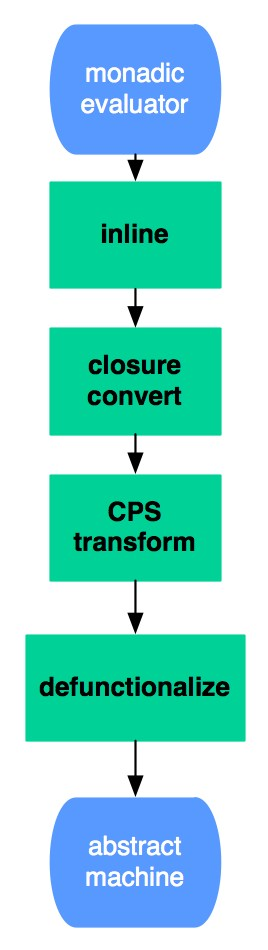
\includegraphics[width=2.3cm, height=7cm]{adm_summary.jpg}

\end{minipage}



\begin{minipage}[r]{7.5cm}


\structure{Producing an abstract machine from a monadic evaluator}{

\normalsize{

\begin{itemize}

  \item{Inline all monadic operations to make computational effects explicit in evaluation}
  \item{Closure convert data types to reduce higher-order data to first-order values}
  \item{CPS transform the evaluator to materialize its control flow as functions "to the rest of the computation" i.e. continuations}
  \item{Defunctionalize continuations to produce a transition system}

\end{itemize}

} % end fontsize

} % end structure

\end{minipage}

\end{tabular*}

\end{frame}

%%%%% slide
\begin{frame}{The Ager-Danvy-Midtgaard (ADM) Transformations}

\center{\emph{\footnotesize{\color{blue}{...defunctionalized continuation-passing evaluators are abstract machines.\cite{ADM_2005}}}}}

\medskip

\begin{tabular*}{15cm}{cc}

\begin{minipage}[]{2.5cm}

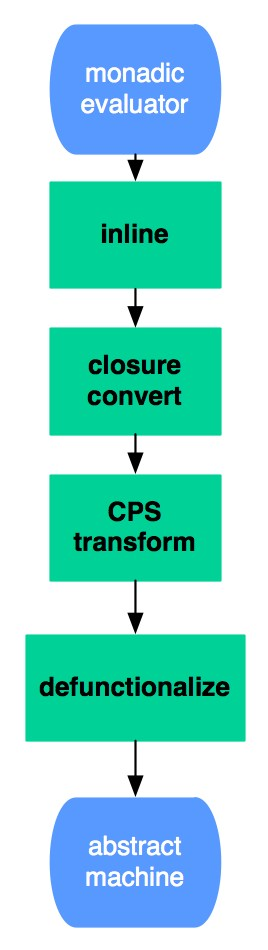
\includegraphics[width=2.3cm, height=7cm]{adm_summary.jpg}

\end{minipage}



\begin{minipage}[r]{7.5cm}

\structure{Producing an abstract machine from the CT evaluator}{

%\normalsize{

\begin{itemize}

  \color{red}{

  \item{Inlining the monadic operations of $R\ a$ simply produces sequential composition}
  \item{Closure conversion is unnecessary because CT has no higher-order data}
  \item{CPS is implicit in the definition of expressible values in CT, i.e. the monad $ResT\ (StateT\ Mem Id) Val$}
  \item{Defunctionalization follows directly, with states delineated by applications of the $Pause$ constructor}
  
  }  % end font color

\end{itemize}

%} % end fontsize

} % end structure

\end{minipage}

\end{tabular*}

\end{frame}




%%%%% slide
\begin{frame}{ADM in Practice: a CT Operational Semantics via DFun}


\structure{Exposing control flow with resumptions}{

\begin{onlinebox}{11cm}

$step_{R}\ k_{0}\ \bigstar_{R}\ step_{R}\ k_{1}\ \bigstar_{R}\ step_{R}\ \bigstar_{R}\ step_R\ k_{2}\ \equiv$

\medskip
%\ \ \ \  \ \ (defn of $\bigstar_R$)\\

$Pause( k_{0}\ \bigstar_{K} \ \eta_{K} (Pause( k_{1}\ \bigstar_{K} \ \eta_{K} (Pause (k_{2}\ \bigstar_{K} \ (\eta_{K} \circ Done))))))$

\end{onlinebox}


} % end structure

\begin{itemize}

  \item{$k_{i}$ are blocks of imperative code}
  \item{$Pause$ delineates blocks from one another}
  \item{When the behavior of a system satisfies this semantics, the argument to $\eta_K$ specifies the remainder of the computation}

\end{itemize}

\structure{Transition system from explicit control flow}{

\begin{onlinebox}{11cm}

$Pause( k_{0}\ \bigstar_{K} \ \eta_{K} (Pause( k_{1}\ \bigstar_{K} \ \eta_{K} (Pause (k_{2}\ \bigstar_{K} \ (\eta_{K} \circ Done))))))$

$\sim$\\
$\lceil \texttt{\_\_k0:}\ \texttt{stmt0;} \dots \texttt{stmtN; jmp \_\_k1}\rceil$\\
$\lceil \texttt{\_\_k1:\ stmt0;} \dots \texttt{stmtM; jmp \_\_k2}\rceil$\\
$\lceil \texttt{\_\_k2:\ stmt0;} \dots \texttt{stmtP; exit\ ret}\rceil$


\end{onlinebox}

} % end structure


\end{frame}



%%%%% slide
\begin{frame}{From RPS to a CT Abstract Machine}

\structure{The RKI abstract machine}{

\begin{small}

\begin{tabular}[t]{|lcr|}\hline

$r$ &$\implies_{init}$& $\langle r, E_{init}, \textsf{nil}\rangle_R$\\
\hline

$\langle Pause\ k, E, R \rangle $&$\implies_R$&$ \langle k, R, E\rangle_K$\\
$\langle BZ\ b\  r\ r\prime,\ E, R\rangle $&$\implies_R$&$ \langle (r, r\prime), b, R, E  \rangle_I$\\
$\langle Loop\ r\ r\prime,E, R\rangle $&$\implies_R$&$ \langle r, E, (r, r\prime)::R\rangle_R$\\
$\langle Done\ v, E, (r, r\prime)::R\rangle$ &$\implies_R$& $\langle r, E[ret \mapsto v], (r, r\prime)::R\rangle_R$\\
$\langle Break\ v, E, (r, r\prime)::R\rangle$ &$\implies_R$&  $\langle r\prime, E[ret \mapsto v], R \rangle_R$\\


\hline
$\langle get_x\ \bigstar_K\ k, R, E \rangle $&$\implies_K$&$ \langle k, E[ret \mapsto \lceil x \rceil]\rangle_K$\\
$\langle put_x\ e\ \bigstar_K\ k, R, E \rangle $&$\implies_K$&$ \langle k, E[x \mapsto \lceil e \rceil,\ ret\mapsto \textsf{nil}]\rangle_K$\\
$\langle \lambda x.k, E \rangle $&$\implies_K$&$ \langle k, E[x \mapsto \lceil ret \rceil]\rangle_K$\\
$\langle \eta_K\ r, R, E \rangle $&$\implies_K$&$ \langle r, E, R\rangle_R$\\
\hline
$\langle (r, r\prime), x, R, E\rangle $&$\implies_I $&$ \langle (r, r\prime), \lceil x \rceil, R, E \rangle_I$\\
$\langle (r, r\prime), 1, R, E \rangle $&$\implies_I $&$ \langle r, E, R\rangle_R$\\
$\langle  (r, r\prime), 0, R, E \rangle $&$\implies_I $&$ \langle r\prime, E, R\rangle_R$\\
\hline
$\langle Done\ x, E, \textsf{nil} \rangle $&$\implies_{halt}$&$ x $

\\
\hline
\end{tabular}

\end{small}

} %end structure


\end{frame}

%%%%% slide
\begin{frame}{From RPS to a CT Abstract Machine}

\structure{The RKI abstract machine}{

\begin{small}

\begin{tabular}[t]{|lcr|}\hline

$r$ &$\implies_{init}$& $\langle r, E_{init}, \textsf{nil}\rangle_R$\\
\hline

$\color{red}{\langle Pause\ k, E, R \rangle }$&$\color{red}{\implies_R}$&$ \color{red}{\langle k, R, E\rangle_K}$\\
$\langle BZ\ b\  r\ r\prime,\ E, R\rangle $&$\implies_R$&$ \langle (r, r\prime), b, R, E  \rangle_I$\\
$\langle Loop\ r\ r\prime,E, R\rangle $&$\implies_R$&$ \langle r, E, (r, r\prime)::R\rangle_R$\\
$\langle Done\ v, E, (r, r\prime)::R\rangle$ &$\implies_R$& $\langle r, E[ret \mapsto v], (r, r\prime)::R\rangle_R$\\
$\langle Break\ v, E, (r, r\prime)::R\rangle$ &$\implies_R$&  $\langle r\prime, E[ret \mapsto v], R \rangle_R$\\

\hline
$\langle get_x\ \bigstar_K\ k, R, E \rangle $&$\implies_K$&$ \langle k, E[ret \mapsto \lceil x \rceil]\rangle_K$\\
$\langle put_x\ e\ \bigstar_K\ k, R, E \rangle $&$\implies_K$&$ \langle k, E[x \mapsto \lceil e \rceil,\ ret\mapsto \textsf{nil}]\rangle_K$\\
$\langle \lambda x.k, E \rangle $&$\implies_K$&$ \langle k, E[x \mapsto \lceil ret \rceil]\rangle_K$\\
$\langle \eta_K\ r, R, E \rangle $&$\implies_K$&$ \langle r, E, R\rangle_R$\\
\hline
$\langle (r, r\prime), x, R, E\rangle $&$\implies_I $&$ \langle (r, r\prime), \lceil x \rceil, R, E \rangle_I$\\
$\langle (r, r\prime), 1, R, E \rangle $&$\implies_I $&$ \langle r, E, R\rangle_R$\\
$\langle  (r, r\prime), 0, R, E \rangle $&$\implies_I $&$ \langle r\prime, E, R\rangle_R$\\
\hline
$\langle Done\ x, E, \textsf{nil} \rangle $&$\implies_{halt}$&$ x $

\\
\hline
\end{tabular}

\end{small}

\medskip

} %end structure

\center{\color{red}{Atomic state delimiter}}


\end{frame}

%%%%% slide
\begin{frame}{From RPS to a CT Abstract Machine}

\structure{The RKI abstract machine}{

\begin{small}

\begin{tabular}[t]{|lcr|}\hline

$r$ &$\implies_{init}$& $\langle r, E_{init}, \textsf{nil}\rangle_R$\\
\hline

$\langle Pause\ k, E, R \rangle$&$\implies_R$&$ \langle k, R, E\rangle_K$\\
$\langle BZ\ b\  r\ r\prime,\ E, R\rangle $&$\implies_R$&$ \langle (r, r\prime), b, R, E  \rangle_I$\\
$\langle Loop\ r\ r\prime,E, R\rangle $&$\implies_R$&$ \langle r, E, (r, r\prime)::R\rangle_R$\\
$\langle Done\ v, E, (r, r\prime)::R\rangle$ &$\implies_R$& $\langle r, E[ret \mapsto v], (r, r\prime)::R\rangle_R$\\
$\langle Break\ v, E, (r, r\prime)::R\rangle$ &$\implies_R$&  $\langle r\prime, E[ret \mapsto v], R \rangle_R$\\

\hline
$\color{red}{\langle get_x\ \bigstar_K\ k, R, E \rangle }$&$\color{red}{\implies_K}$&$\color{red}{ \langle k, E[ret \mapsto \lceil x \rceil]\rangle_K}$\\
$\color{red}{\langle put_x\ e\ \bigstar_K\ k, R, E \rangle}$&$\color{red}{\implies_K}$&$\color{red}{ \langle k, E[x \mapsto \lceil e \rceil,\ ret\mapsto \textsf{nil}]\rangle_K}$\\
$\color{red}{\langle \lambda x.k, E \rangle }$&$\color{red}{\implies_K}$&$\color{red}{ \langle k, E[x \mapsto \lceil ret \rceil]\rangle_K}$\\
$\color{red}{\langle \eta_K\ r, R, E \rangle }$&$\color{red}{\implies_K}$&$\color{red}{ \langle r, E, R\rangle_R}$\\
\hline
$\langle (r, r\prime), x, R, E\rangle $&$\implies_I $&$ \langle (r, r\prime), \lceil x \rceil, R, E \rangle_I$\\
$\langle (r, r\prime), 1, R, E \rangle $&$\implies_I $&$ \langle r, E, R\rangle_R$\\
$\langle  (r, r\prime), 0, R, E \rangle $&$\implies_I $&$ \langle r\prime, E, R\rangle_R$\\
\hline
$\langle Done\ x, E, \textsf{nil} \rangle $&$\implies_{halt}$&$ x $

\\
\hline
\end{tabular}

\end{small}

\medskip

} %end structure

\center{\color{red}{Imperative actions}}


\end{frame}


%%%%% slide
\begin{frame}{From RPS to a CT Abstract Machine}

\structure{The RKI abstract machine}{

\begin{small}

\begin{tabular}[t]{|lcr|}\hline

$r$ &$\implies_{init}$& $\langle r, E_{init}, \textsf{nil}\rangle_R$\\
\hline

$\langle Pause\ k, E, R \rangle $&$\implies_R$&$ \langle k, R, E\rangle_K$\\
$\langle BZ\ b\  r\ r\prime,\ E, R\rangle $&$\implies_R$&$ \langle (r, r\prime), b, R, E  \rangle_I$\\
$\color{red}{\langle Loop\ r\ r\prime,E, R\rangle }$&$\color{red}{\implies_R}$&$\color{red}{ \langle r, E, (r, r\prime)::R\rangle_R}$\\
$\color{red}{\langle Done\ v, E, (r, r\prime)::R\rangle}$ &$\color{red}{\implies_R}$& $\color{red}{\langle r, E[ret \mapsto v], (r, r\prime)::R\rangle_R}$\\
$\color{red}{\langle Break\ v, E, (r, r\prime)::R\rangle}$ &$\color{red}{\implies_R}$&  $\color{red}{\langle r\prime, E[ret \mapsto v], R \rangle_R}$\\


\hline
$\langle get_x\ \bigstar_K\ k, R, E \rangle $&$\implies_K$&$ \langle k, E[ret \mapsto \lceil x \rceil]\rangle_K$\\
$\langle put_x\ e\ \bigstar_K\ k, R, E \rangle $&$\implies_K$&$ \langle k, E[x \mapsto \lceil e \rceil,\ ret\mapsto \textsf{nil}]\rangle_K$\\
$\langle \lambda x.k, E \rangle $&$\implies_K$&$ \langle k, E[x \mapsto \lceil ret \rceil]\rangle_K$\\
$\langle \eta_K\ r, R, E \rangle $&$\implies_K$&$ \langle r, E, R\rangle_R$\\
\hline
$\langle (r, r\prime), x, R, E\rangle $&$\implies_I $&$ \langle (r, r\prime), \lceil x \rceil, R, E \rangle_I$\\
$\langle (r, r\prime), 1, R, E \rangle $&$\implies_I $&$ \langle r, E, R\rangle_R$\\
$\langle  (r, r\prime), 0, R, E \rangle $&$\implies_I $&$ \langle r\prime, E, R\rangle_R$\\
\hline
$\langle Done\ x, E, \textsf{nil} \rangle $&$\implies_{halt}$&$ x $

\\
\hline
\end{tabular}

\end{small}

} %end structure

\medskip

\center{\color{red}{Iteration}}



\end{frame}




%%%%% slide
\begin{frame}{Example: Defunctionalizing a Trivial Kernel}

\begin{structure}{Dumb Little Kernel}

\begin{footnotesize}

\begin{tabular}[t]{lll}


\texttt{main =}&\texttt{loop\_R}\\

&\texttt{($\backslash$ r\ ->}\\

&&\texttt{case\ r\ of}\\
&&\texttt{Pause\ x\ -> step\_R\ x\ >>=\ $\backslash$r0\ ->\  return\ r0}\\
&&\texttt{Done\ v\ -> break\_R\ v}\\

&\texttt{)\ phi}\\

\end{tabular}

\texttt{phi\ =}\\
\texttt{step\_R(get\ G\ >>= $\backslash$v\ ->}
\texttt{put\ G\ (v + 1)\ >>\ return\ v)\ >>=\ $\backslash$v\ -> return\ v}\\

\end{footnotesize}

\end{structure}

\bigskip

\begin{structure}{Dumb Little Assembly Fragment}

\begin{footnotesize}


\begin{tabular}[t]{llll}

\begin{minipage}[l]{2cm}
\begin{texttt}
\_\_main:\\
r\ :=\ \_\_phi\\
s\ :=\ 1\\
\_\_loop:\\
tst\ s\\
bz\ \_\_case1\\
\_\_case0:\\
jsr r\\
jmp \_\_loop\\

\end{texttt}

\end{minipage}



&

\begin{minipage}[l]{2.5cm}

\begin{texttt}
\_\_case1:\\
ret\ :=\ ret\\
jmp\ \_\_loop\_exit\\
\_\_loop\_exit:\\
halt
\end{texttt}

\end{minipage}


&

\begin{minipage}[l]{2cm}

\begin{texttt}
\_\_phi:\\
s\ := 1\\
ret\ :=\ G\\
v\ :=\ ret\\
G\ :=\ v\ +\ 1\\
ret\ := v\\
r\ := \_\_phi0\\
rts\\
\end{texttt}

\end{minipage}

&
\begin{minipage}[l]{2cm}

\begin{texttt}
\_\_phi0:\\
ret\ := v\\
s\ := 0\\
rts\\
\end{texttt}

\end{minipage}


\end{tabular}

\end{footnotesize}


\end{structure}


\end{frame}



%%%%% slide
\begin{frame}{Ideal Target: A Typed Assembly Language (TAL)}

\begin{structure}{A typed assembly language of linear continuations \cite{Zdancewic_Meyers_2002}}

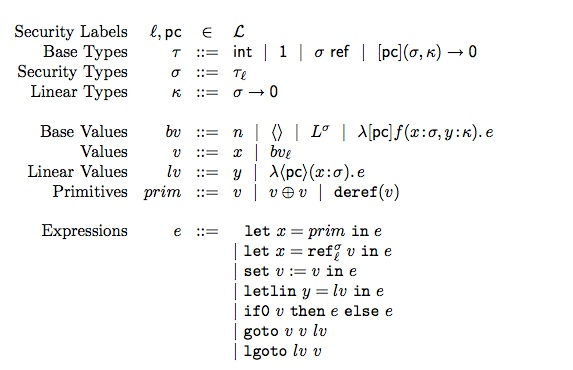
\includegraphics[width=8cm]{zd_syntax.jpg}

\end{structure}

\begin{structure}{Next steps}

\begin{itemize}
\item{Memory safety via low-level type system}
\item{Operationalizing memory maps}
\end{itemize}

\end{structure}


\end{frame}




%%%%% slide
\begin{frame}{Verification Objective: A Simulation Relation Between CT and TAL}


\begin{structure}{Goal: implement this relation}

\center{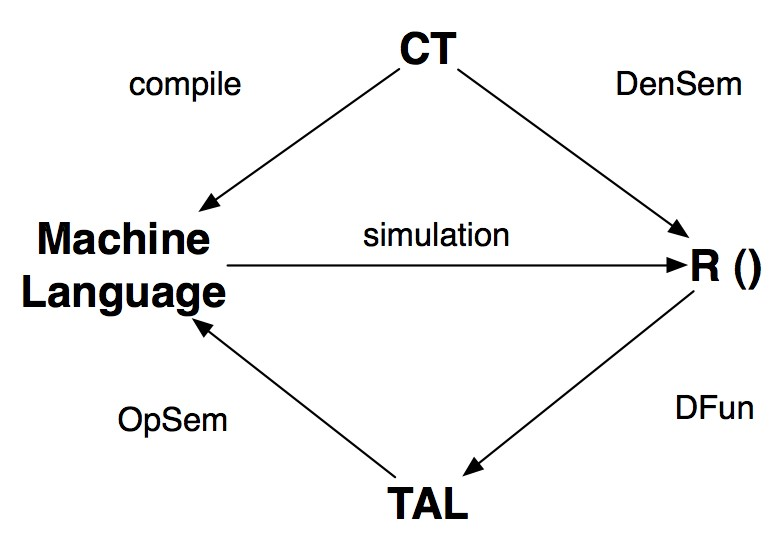
\includegraphics[width=6.5cm]{correctness.jpg}}

\begin{itemize}

\item{CT denotes resumptions, i.e. explicit action sequences}
\item{R defunctionalizes to transition systems with mutable state}
\item{TAL realizes an operational semantics, simulates resumptions}
\item{That's model-driven engineering}

\end{itemize}

\end{structure}

\end{frame}

%%%%% slide
\begin{frame}{"With just one line of code, HASK Lab rips all these signed, big-budget motherf*ckers."\\ Questions?}


\includegraphics[width=10cm]{funcrusher.jpg}

\end{frame}


%%%% bibliography
\bibliographystyle{plain}
\bibliography{talk_2010.08.13}




\end{document}